%!TEX root = PhD_Thesis.tex
\chapter[Estimation and Control]{Estimation and Control for 3D-Ultrasound-Guided Needle Steering}

\section{Introduction}
The previous two chapters described methods for ultrasound imaging and needle design, both intended to make image-guided needle steering practical in biological tissue. In this chapter, techniques from the previous chapters are combined into a complete system for 3D-ultrasound-guided needle steering. The system is validated in simulated clinical scenarios in bench-top and animal models. 

Although ultrasound has many advantages as an imaging modality, it produces noisy data compared to CT or MR imaging. This is especially true when using high-frequency vibration and Doppler ultrasound imaging to segment a curved needle, as described in Chapter 2. While we demonstrated that this approach can reveal the curved shape of the needle, the resulting measurement error is large relative to the desired precision of percutaneous ablation. (Clinicians using medical image guidance systems can manually position needle tips within approximately 2~mm of a target in similar interventions~\cite{Crocetti2008}.) Manual localization of a steerable needle in ultrasound data, which is described in this chapter, also involves large amounts of measurement noise. A further difficulty is that ultrasound imaging provides infrequent measurements. This is a result of the low volumetric framerate in the case of 3D Doppler imaging, and the time-consuming nature of manual localization. 

In this chapter, to attain clinically relevant targeting precision using sparse, noisy measurements, we apply a model-based recursive estimation scheme known as an unscented Kalman filter (UKF). This filter relies on experimental quantification of process and measurement noise for ultrasound-guided needle steering in biological tissue, which was performed using an electromagnetic tracking system as a reference.
 
This chapter is divided into three main sections. Section~\ref{sec:UKF} describes the UKF estimation scheme. Section~\ref{sec:AutonomousControl} describes an implementation autonomous image-guided needle control based on the UKF. Section~\ref{sec:HumanInTheLoopControl} describes human-in-the-loop control based on the UKF.

%======================================================================
\section[UKF Estimation Scheme]{Unscented Kalman Filter Estimation Scheme}
%======================================================================
\label{sec:UKF}
\subsection{Needle Steering Model}
Our kinematic model of needle steering is based on the unicycle model~\cite{Webster2006}; we assume the needle travels along curved paths that are tangent to each other. To begin, we define the needle tip frame. As shown in Fig.~\ref{fig:NeedleKinematics}, this frame is attached to the tip of the steerable needle, and oriented so that its \textit{z}-axis is tangent to the needle at the tip, and its \textit{y}-axis points towards the center of curvature. In this model, the state of the needle is described by the pose of the needle tip frame relative to a reference frame, in our case the 3D ultrasound frame or robot frame. 

\subsubsection{Needle State Representation}
Needle tip position is represented by a vector ${p} \in \mathbb{R}^3$. There are several possible representations of tip orientation, including quaternions, Euler angles, and axis-angle rotation vectors. We have elected to use a rotation matrix ${R} \in \textrm{SO(3)}$. This is a singularity-free representation. To describe differential rotations, we will frequently use the equivalent axis-angle rotation vector $r \in \textrm{so(3)}$, which can be calculated directly from ${R}$. The state ${x}$ is thus defined as
\begin{align}
{x} = \{p \in \mathbb{R}^3, R \in \textrm{SO(3)}\}
\end{align}

\begin{figure*}[!t]
\centering
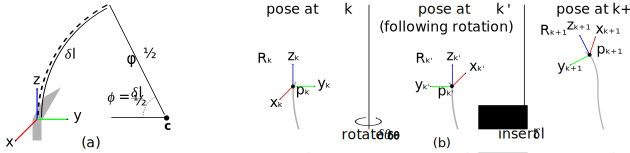
\includegraphics[width=\textwidth]{Images/Chapter4/NeedleKinematics/NeedleKinematics}%
\caption[Kinematic model of needle steering used in image-guided control]{Kinematic model of needle steering~\cite{Webster2006} used in image-guided control: (a) Needle tip frame. The $z$-axis is tangent to the needle at the tip (ignoring the bevel or prebent section), the $y$-axis points towards the center of curvature. The needle path is an arc within the $y$-$z$ plane with radius $\rho$ and arc length $\delta l$. (b) Progression of the needle tip frame during steering. The steerable needle insertion is divided into increments, with incremental needle rotation angle ($\delta\theta$), incremental insertion distance ($\delta l$) and radius of curvature ($\rho$) updated as command inputs between increments. These command inputs define the transition of state vector ${x}$.}
\label{fig:NeedleKinematics}
\end{figure*}

\subsubsection{State Transition Model}
Based on the kinematic model of needle steering~\cite{Webster2006}, we define the transition of needle state to the next time interval, ${x_{k+1}}$, as a function of the current state, ${x_{k}}$, a vector of command inputs, ${u_{k}}$, and a vector of process noise, ${w}$:
\begin{align}
{x_{k+1}} = f({x_k}, {u_k}, {w}).
\end{align}
In our model, we divide needle steering into incremental insertions. Command inputs are applied between incremental insertions, and include change in needle base rotation $\delta\theta$, incremental insertion distance $\delta l$, and radius of incremental needle path $\rho$:
\begin{align}
{u} = \begin{bmatrix} \delta\theta & \delta l & \rho\end{bmatrix}^{\text{T}}.
\end{align}
The radius of the needle path can be experimentally measured as described in the previous chapters. The radius can also be adjusted using duty cycling~\cite{Minhas2007}, a control approach that uses short, variable periods of insertion with and without rotation to adjust needle curvature from maximum curvature to straight. System variability is modeled using nonadditive Gaussian noise in the state transition model. The noise ${w}$ can be separated into a position component, ${p_w} \in \mathbb{R}^3$, and an orientation component, ${r_w} \in SO(3)$. The index $k$ is omitted from the vector ${w}$ to signify the random nature of the vector.

The state transition function $f$ can be viewed as a transformation of the tip frame, as shown in Fig.~\ref{fig:NeedleKinematics}. The needle tip frame at time ${k}$ has pose defined by ${p_{k}}$ and ${R_{k}}$. The needle tip frame is first rotated about its $z$-axis by $\delta\theta$ to yield the rotated tip frame:
\begin{align}
{R_{k'}} = {R_{k}}{Rz}(\delta\theta).
\end{align}
The needle is then inserted a distance $\delta l$, with the tip following a circular path of radius $\rho$. From the definition of the tip frame shown in Fig.~\ref{fig:NeedleKinematics}, we know that the needle path will lie in the $y$-$z$ plane of the rotated frame defined by ${R_{k'}}$. The position of the needle tip after insertion relative to the rotated frame can be found directly from the geometry of the circular path:
\begin{align}
{^{k'}p_{k+1}} = \begin{bmatrix}0\\ \rho(1-\cos(\frac{\delta l}{\rho})) \\ \rho\sin(\frac{\delta l}{\rho})\end{bmatrix}.
\end{align}
Transforming this vector into the world frame, and including process noise yields an expression for $p_{k+1}$:
\begin{align}
{p_{k+1}} = {R_{k}}{Rz}(\delta\theta){^{k'}p_{k+1}}+{p_k} +{p_w}.
\end{align}
%\begin{align}
%\begin{array} {lcl} {p_{k+1}} & = & \bm{R_{k}}{Rz}(\delta\theta){^{k'}p_{k+1}}+{p_k} +{p_w} \\ & = & {R_{k}}{Rz}(\delta\theta)\begin{bmatrix}0\\ \rho(1-\cos(\frac{l}{\rho})) \\ \rho\sin(\frac{l}{\rho})\end{bmatrix}+{p_k} +{p_w}.\end{array}
%\end{align}
The orientation of the tip frame after insertion can be defined using the same rotation matrices. Similar to other studies that have applied Kalman filters to orientation representations~\cite{Kraft2003}, we include orientation noise as an initial disturbance to the state vector, ${R_w}$.
The updated tip frame orientation is thus
\begin{align}
{R_{k+1}} = {R_{k}}{R_w}{Rz}(\delta\theta){Rx}\left(\begin{matrix}-\frac{\delta l}{\rho}\end{matrix}\right).
\end{align}
The vector ${r_{k+1}}$ is the rotation vector equivalent of ${R_{k+1}}$.

\subsubsection{Measurement Model}
Based on our 3D ultrasound needle segmentation method~\cite{Adebar2013}, we define the measurement model as full-state feedback with additive measurement noise vector ${v}$:
\begin{align}
{z_{k}} = {x_k} + {v}.
\end{align}
This model assumes that the automatic or manual segmentation method can measure the full 6DOF pose of the needle tip frame. Although rotation around the axis of a needle can not generally be resolved by 3D ultrasound, in the case of a curved steerable needle we can use the direction of needle curvature to estimate the $y$-axis of the needle frame.

\subsection{Unscented Kalman Filter}
The unscented Kalman Filter is an extension of the classical Kalman filter to nonlinear systems, and uses a set of sampled points around a mean value to represent distributions~\cite{Julier1997}. For brevity, we omit a detailed description of the typical UKF, and refer the reader to~\cite{Thrun2005} for a complete explanation. Our implementation of the UKF follows the original description of the algorithm~\cite{Julier1997}, with several modifications as described below. 

\subsubsection{Calculation of the Mean and Covariance}
The first modification is our method for calculating the mean $\overline{x}$ and covariance $P$ of a set of states $x_0 \dots x_k$. In the UKF, this method is used to recover the mean and covariance of the state estimate from a set of transformed sigma points. Normally in a UKF, the state exists in a vector space, and can be represented by a vector $x \in R^n$. The mean of a set of vector states can be calculated as the sum of the states divided by the size of the set,
\begin{align}
\overline{x} = \frac{1}{k}\sum\limits_{i=1}^{k} x_i,
\end{align}
\noindent 
while the corresponding covariance can be calculated as:
\begin{align}
P = \frac{1}{k}\sum\limits_{i=1}^{k} (x_i-\overline{x})(x_i-\overline{x})^T.
\end{align}
\noindent
Our state includes the 3D position of the needle tip, represented by a vector ${p} \in \mathbb{R}^3$, and the 3D orientation of the needle tip, represented by a matrix ${R} \in \mathbb{SO}^3$. Because orientation is periodic, it is not possible to calculate the mean state or covariance using the above formulae. Instead, we use the iterative gradient descent approach proposed by Kraft~\cite{Kraft2003}. 

NEED TO FINISH THIS.

Given a set of state measurements $x_0 \dots x_k$, with each $x_i = \{p_i,R_i\}$, we calculate the mean position as:
\begin{align}
\overline{p} = \frac{1}{k}\sum\limits_{i=1}^{k} p_i.
\end{align}
We then calculate the set of equivalent rotation vector representations $r_i \dots r_k$.

\subsubsection{Injection of Process and Measurement Noise}
Since the effect of process noise on the state transition is nonadditive, we include the noise covariance matrix $Q$ (described in the next section) in the generation of the Sigma points, as suggested in
 
%======================================================================
\section[Autonomous Control using the UKF]{Autonomous Control using the Unscented Kalman Filter}
%======================================================================
\label{sec:AutonomousControl}



%======================================================================
\section[Human-in-the-Loop Control using the UKF]{Human-in-the-Loop Control using the Unscented Kalman Filter}
%======================================================================
\label{sec:HumanInTheLoopControl}